\chapter{Software Architecture Design}
\label{chap:software-architecture-design}

\section{Domain Model}
\label{section:domain-model}
The domain model of Spell Splash illustrates the core components and interactions of the game—players, 
vocabulary words, quizzes, challenges, and rewards. It demonstrates how gameplay supports vocabulary 
learning through engaging activities like battles and puzzles, connecting educational goals with interactive 
mechanics to make English learning more effective and enjoyable.
\begin{figure}[H]
    \centering
    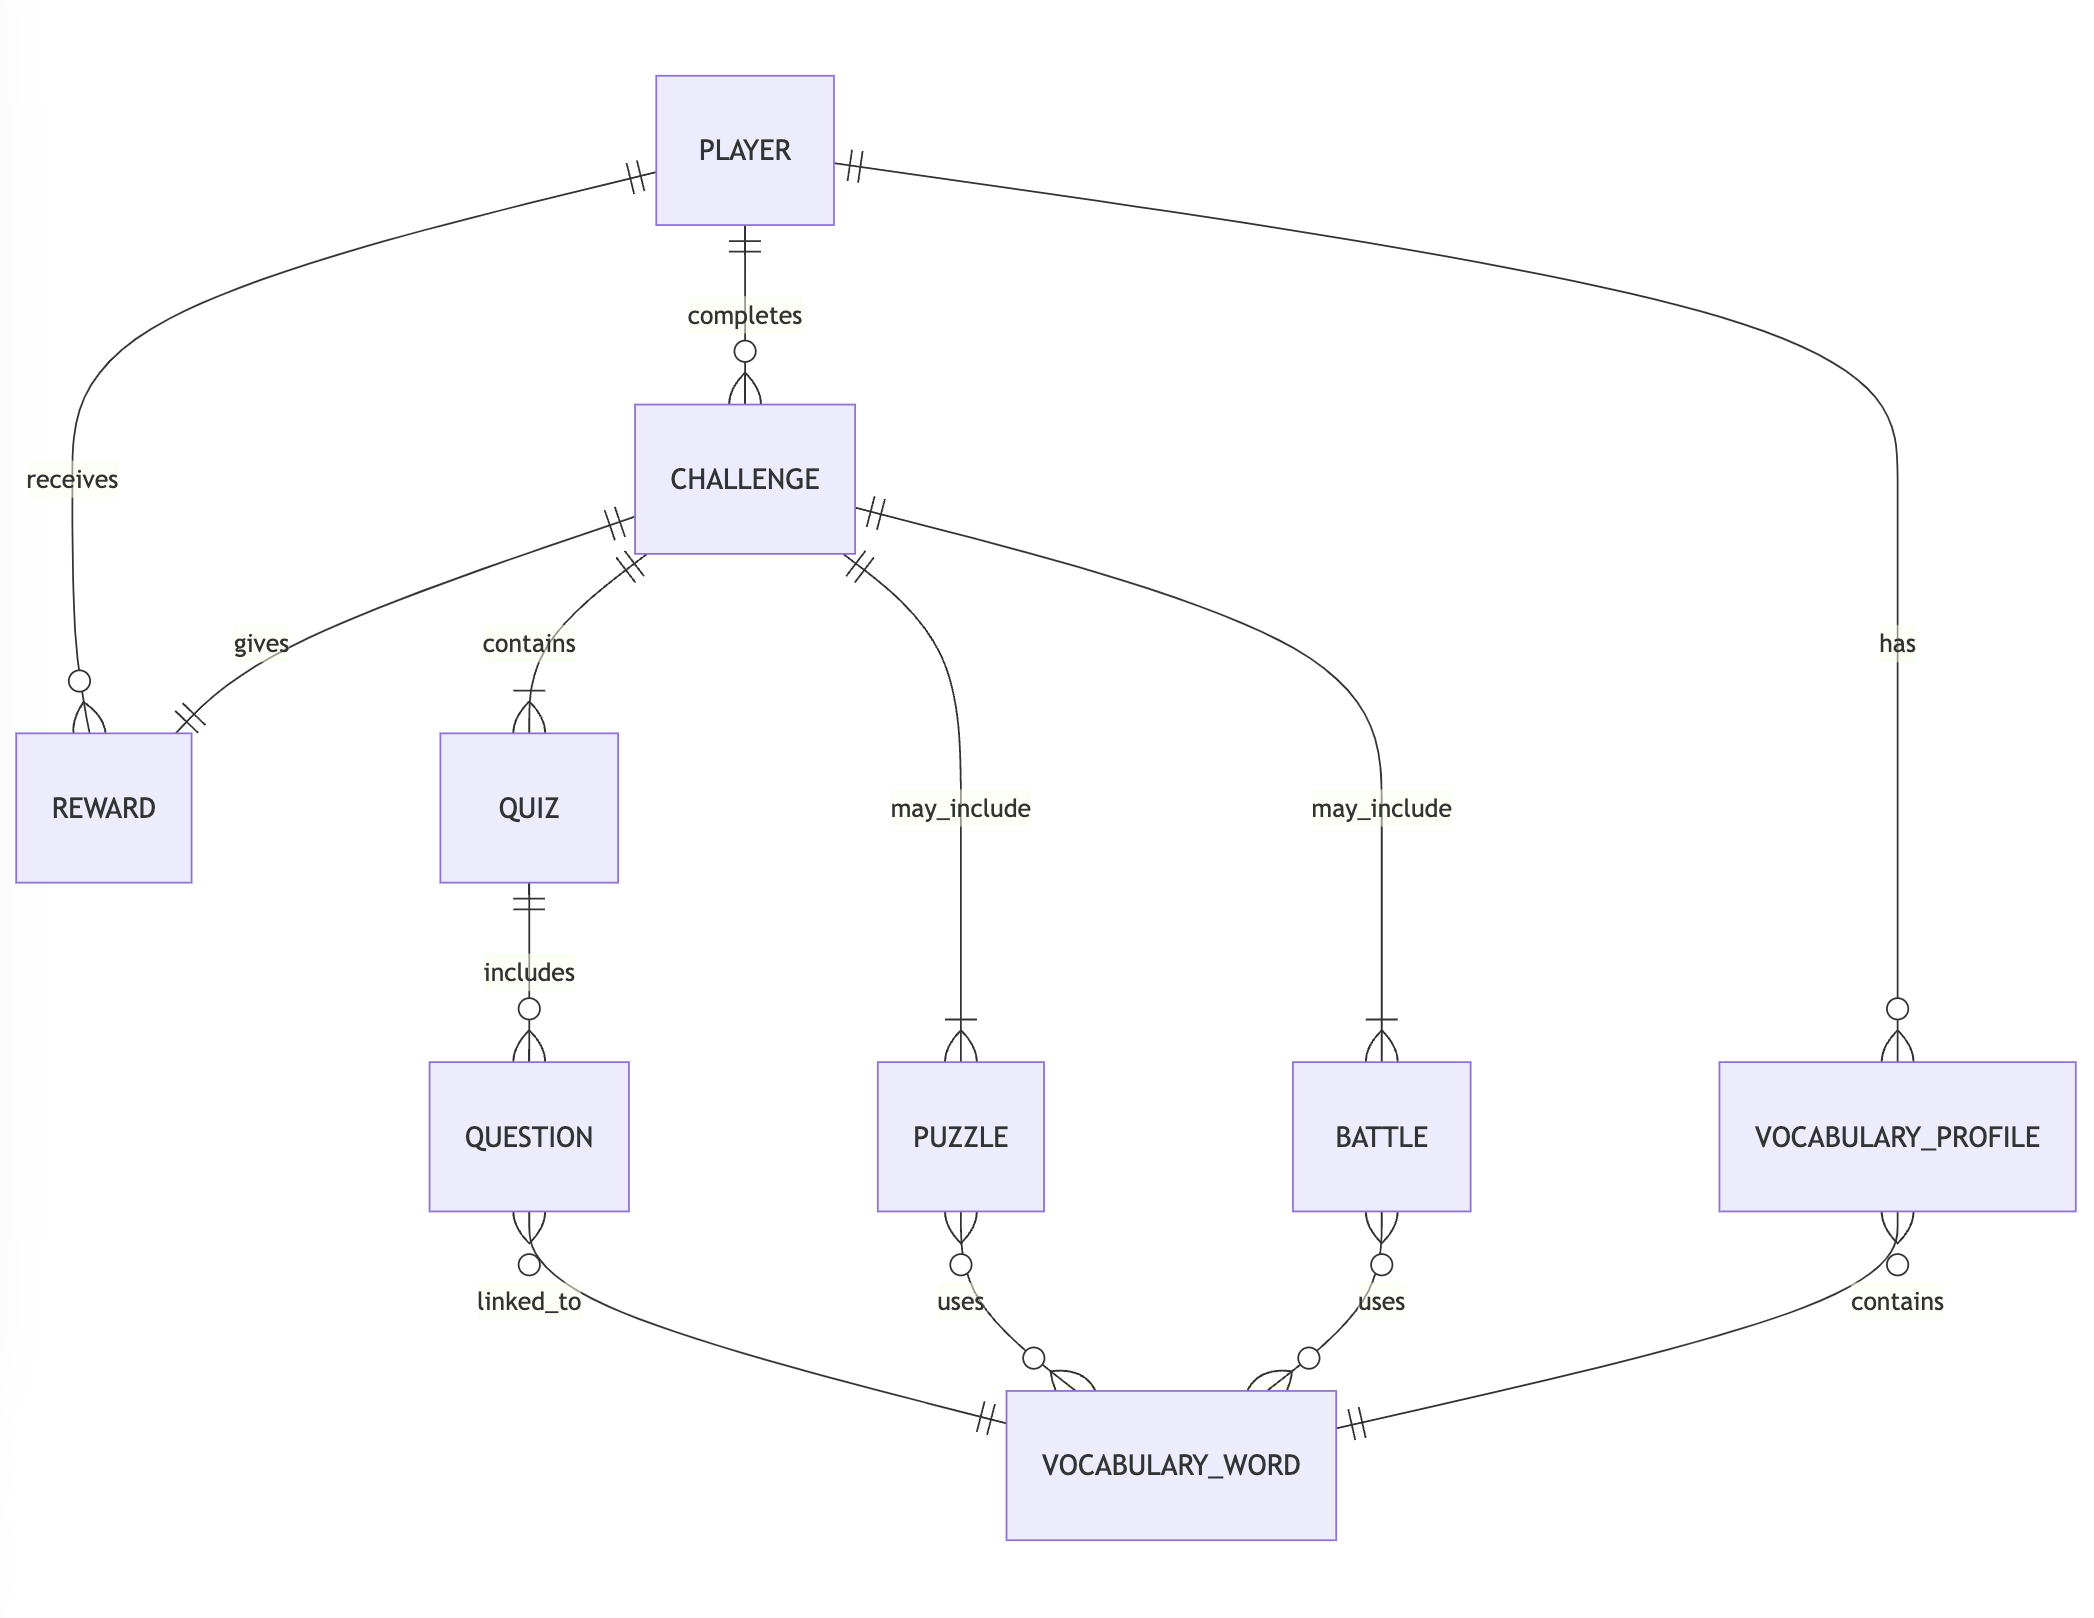
\includegraphics[width=0.85\textwidth]{assets/ku/er_diagram.png}
    \caption{Domain Model of Spell Splash}
    \label{fig:domain-model}
\end{figure}

\section{Design Class Diagram}
\label{section:design-class-diagram}
The Design Class Diagram defines the structure of the Spell Splash system, specifying 
key classes involved in gameplay, vocabulary learning, and player progression. It provides 
a blueprint for how the game's components interact and support both educational and entertainment goals.

\vspace{1em}

\begin{enumerate}
    \item \textbf{Player}\\
    The user of the game who progresses through challenges, earns rewards, and builds vocabulary knowledge. 
    Each player has a profile containing their experience level, completed challenges, and a personalized vocabulary list that tracks learning progress.

    \item \textbf{Challenge}\\
    A general structure representing a learning activity in the game. 
    It serves as the base class for various challenge types such as quizzes, puzzles, and battles. 
    Upon completion, challenges grant players rewards and contribute to their learning progress.

    \item \textbf{Quiz}\\
    A challenge type that consists of multiple-choice questions testing vocabulary understanding. 
    Each quiz is composed of a set of questions, which are randomly selected or generated based on the player's vocabulary level.

    \item \textbf{Puzzle}\\
    A mini-game challenge requiring players to solve vocabulary-based problems or patterns. 
    These challenges reinforce word usage and meaning in fun, creative ways.

    \item \textbf{Battle}\\
    A turn-based combat scenario where correct answers to vocabulary questions translate into in-game attacks. 
    This gamified interaction boosts motivation and retention through high engagement.

    \clearpage

    \item \textbf{Question}\\
    A single quiz item that includes a question prompt, multiple answer options, and one correct answer. 
    Each question is tied to a specific vocabulary word and tests the player's understanding of its meaning or usage.

    \item \textbf{VocabularyWord}\\
    The core learning unit of the game, representing English words the player is expected to master. 
    It includes attributes like word, meaning, pronunciation, and difficulty level. 
    VocabularyWords appear across quizzes, puzzles, and battles.

    \item \textbf{Reward}\\
    A bonus or incentive given to players after completing a challenge. 
    Rewards may include experience points, virtual currency, or items used in gameplay, encouraging continued participation.

    \item \textbf{VocabularyProfile}\\
    A personalized collection of words the player has learned or is currently learning. 
    This class tracks progress and helps adapt the game’s difficulty and content to suit individual learners.
\end{enumerate}

\clearpage

\begin{figure}[H]
    \centering
    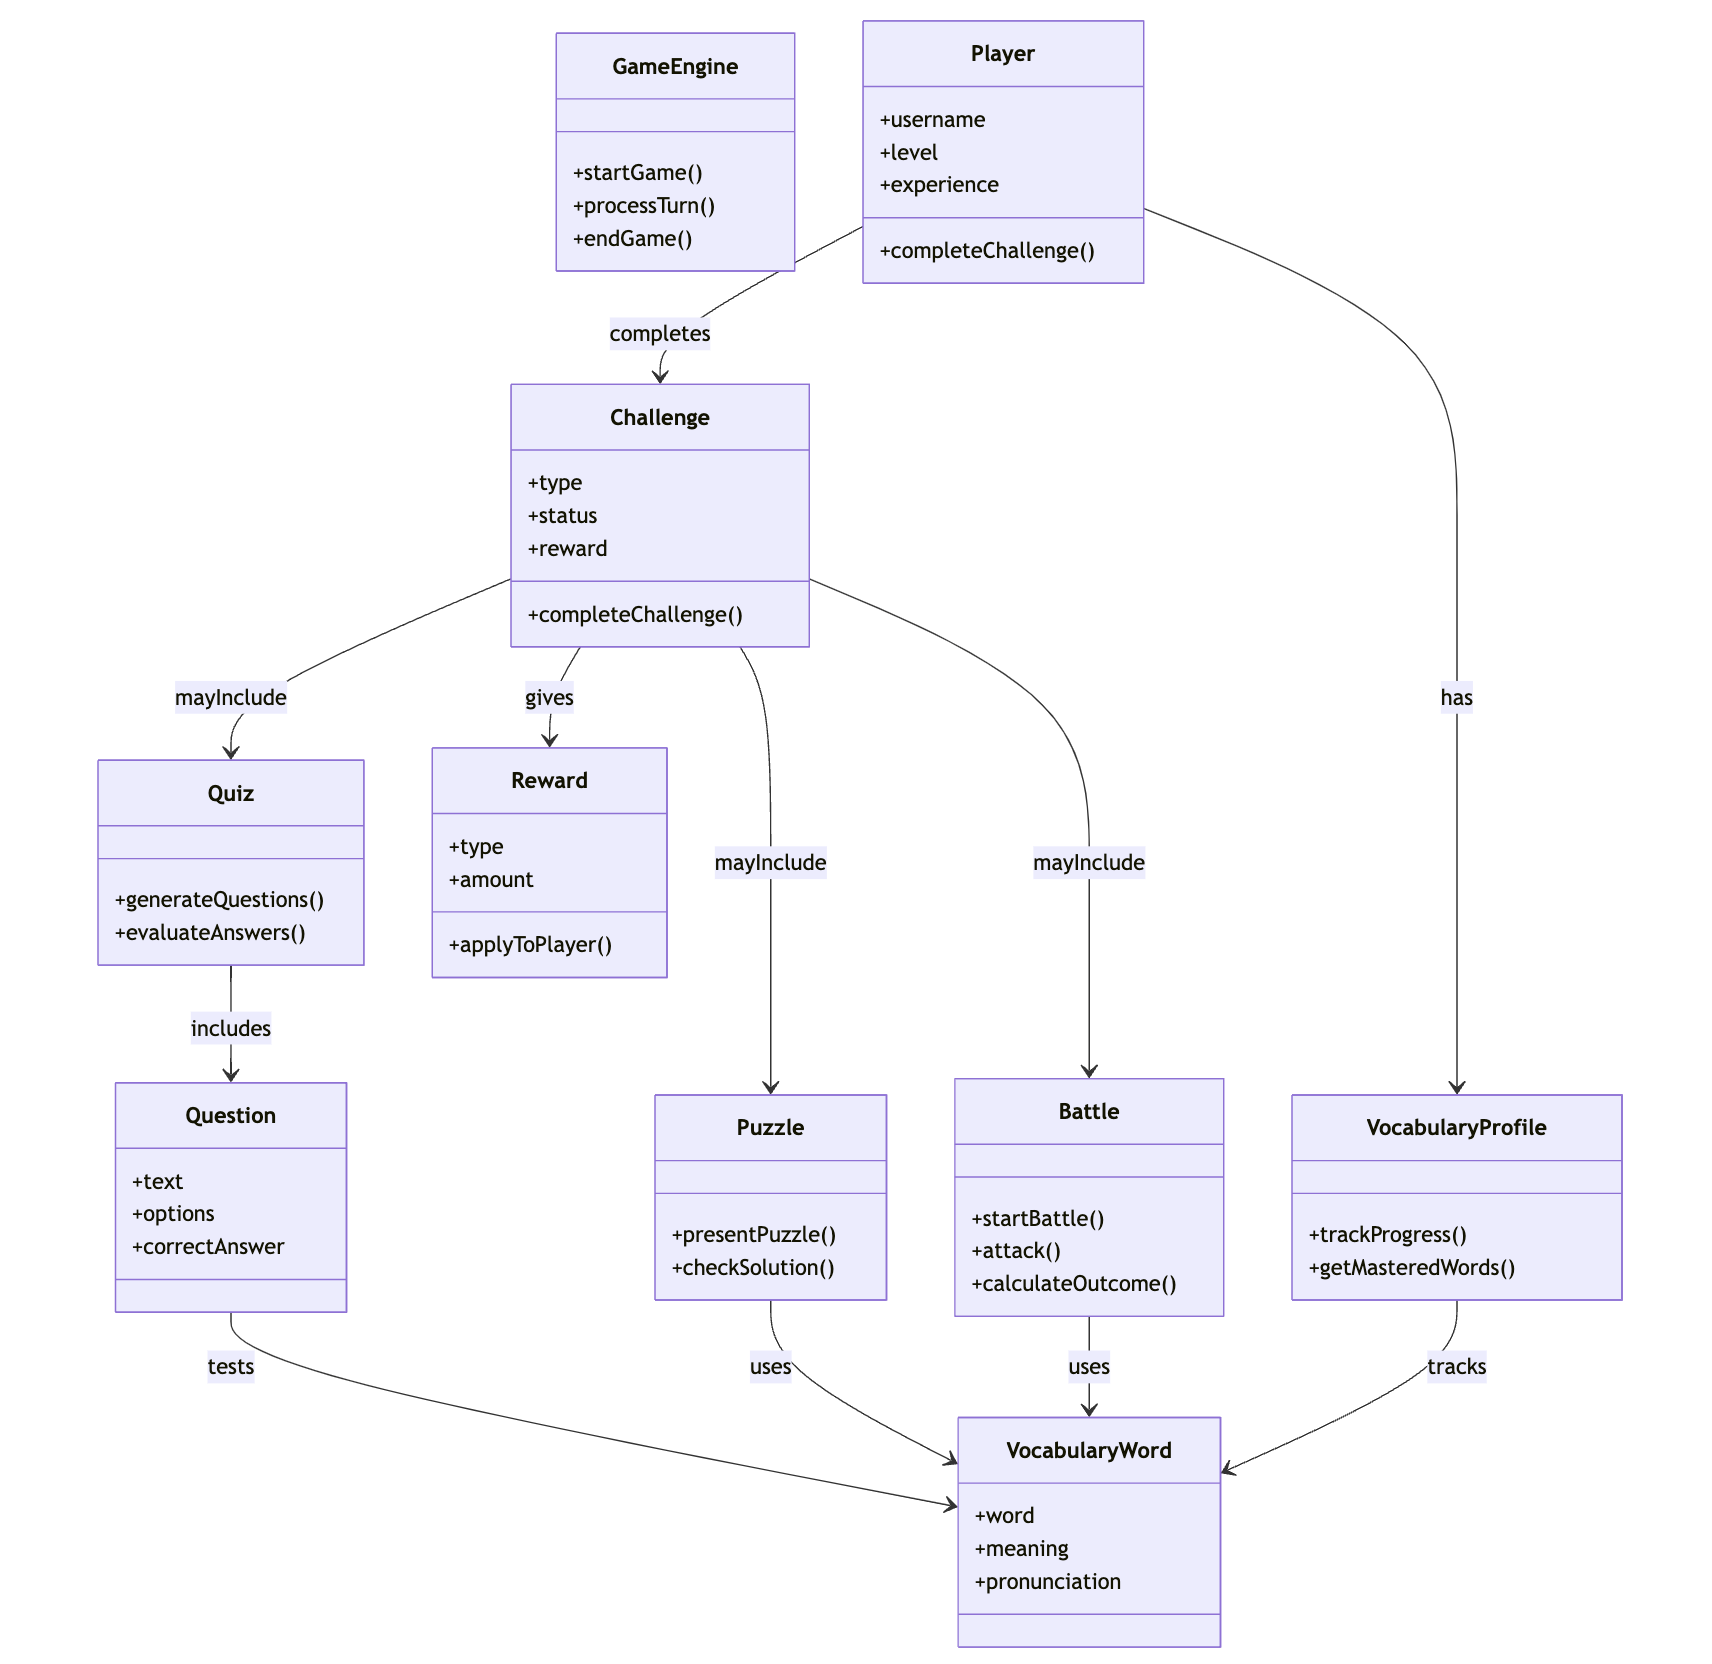
\includegraphics[width=1\textwidth]{assets/ku/class_diagram.png}
    \caption{Class Diagram of Spell Splash}
    \label{fig:design-class-diagram}
\end{figure}

\clearpage

\section{Sequence Diagram}
\label{section:sequence-diagram}

A player initiates a battle. During the battle, the system presents vocabulary questions. 
The player's answers determine the outcome of the battle (correct = damage to enemy). 
Upon winning, the player earns a reward and their vocabulary progress is updated.

\vspace{1em}

\textbf{Scenario: A player completes a vocabulary battle challenge}
\begin{enumerate}
    \item The player starts a new battle from the main game menu.
    \item The game engine requests a new challenge from the challenge manager.
    \item The challenge manager creates and initializes a battle challenge.
    \item The battle system requests a vocabulary word and generates a question.
    \item The system presents the question to the player.
    \item The player submits an answer.
    \item The system checks the answer for correctness.
    \item If correct, the system triggers a player attack; otherwise, the enemy attacks.
    \item Steps 4 to 8 repeat until the battle ends.
    \item The game engine determines the battle outcome (win or lose).
    \item If the player wins, the reward system grants experience or items.
    \item The player's vocabulary profile is updated based on the words used in the battle.
\end{enumerate}

\clearpage

\begin{figure}[H]
    \centering
    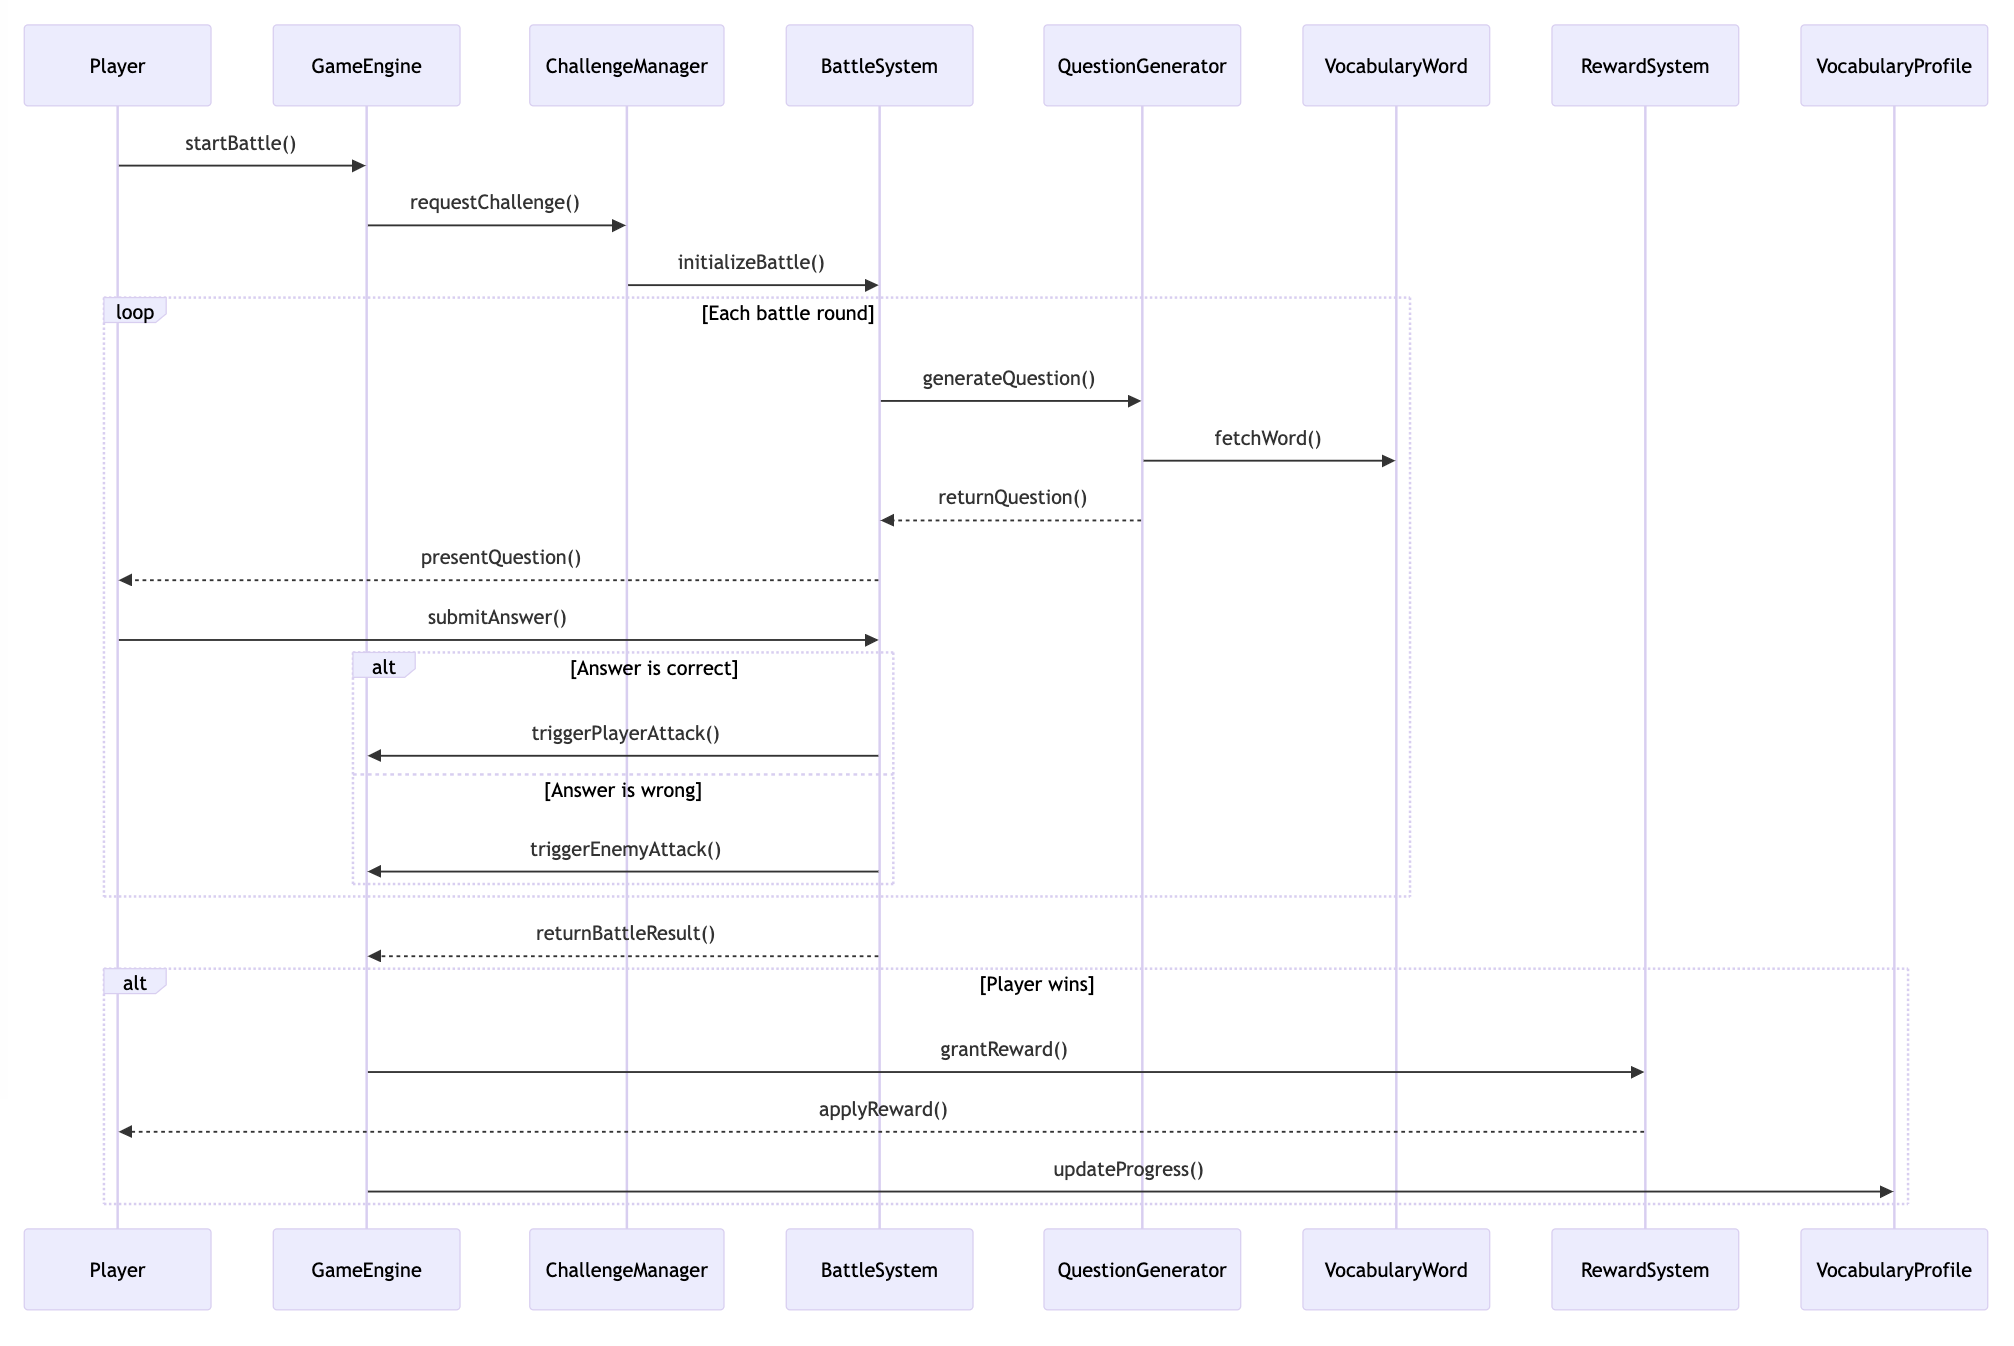
\includegraphics[width=1\textwidth]{assets/ku/sequence_diagram.png}
    \caption{Sequence Diagram of Spell Splash}
    \label{fig:sequence-diagram}
\end{figure}

\clearpage

\section{Algorithm}
\label{section:algorithm}
<TIP: Optional, If you are working on a research project that proposes a new
algorithm, you can describe your algorithm here. It can be in the form of
pseudocode or any diagram that you deem appropriate./>